%%%%%%%%%%%%%%%%%%%%%%%%%%%%%%%%%%%%%%%%%%%%%%%%%%%%%%%%%%%%%%%%%%%%%%%%%%%
%%
%%  ap-programs.tex
%%
%%  Created: Fri Oct 10 14:24:37 1997
%%  Author.: Jose Carlos Gonzales
%%  Notes..:
%%          
%%-------------------------------------------------------------------------
%% Filename: $RCSfile$
%% Revision: $Revision$
%% Date:     $Date$
%%%%%%%%%%%%%%%%%%%%%%%%%%%%%%%%%%%%%%%%%%%%%%%%%%%%%%%%%%%%%%%%%%%%%%%%%%%


\chapter{Descripci\'on t\'ecnica de los programas para el an\'alisis de 
  datos de \MC}
\label{appendix:programs}

El programa para la generaci'on de nuestros datos de \MC (casc'adas
atmosf'ericas iniciadas por rayos c'osmicos y gamma) y su modo de
operaci'on ya fue brevemente descrito en el cap'itulo
\ref{chapter:simshowers} y el ap'endice 
\ref{appendix:corsika}. Asimismo, los programas para el an'alisis de
estos datos fueron mencionados y su ejecuci'on explicada en el
cap'itulo \ref{chapter:simmagic}. En este ap'endice hablaremos de
algunas cuestiones t'ecnicas de estos 'ultimos programas.

\afterpage{\clearpage}


\section{Definici\'on del telescopio}
\label{sec:ctdef}

Dos son los programas principales para el an'alisis de los datos de
\MC: \reflector y \camera. El primero intenta simular los espejos, la
montura y las caracter'isticas 'opticas de \MAGIC, mientras que el
segundo se encarga de la simulaci'on de la c'amara de \MAGIC. En
realidad, esto no es rigurosamente cierto, en el sentido de que su
proceso de simulaci'on no se restringe al telescopio \MAGIC: ambos
c'odigos toman como parte de sus datos de entrada lo que hemos dado en
denominar \emph{Fichero de definici'on del CT}.  Este fichero contiene
una lista de comandos (en ingl'es), acompa~nados a veces de valores,
en la forma
%
\begin{verbatim}
   <comando>   [ <valor1> [ <valor2> ... ] ]
\end{verbatim}
%
Aquellas l'ineas que comiencen con el s'imbolo ``\texttt{\#}'' son
tratadas como l'ineas que contienen comentarios, e ignoradas.  Los
comandos actualmente soportados (comprendidos por \reflector) se
muestran en la tabla \ref{tbl:ctdefkeywords}.  Las unidades de
magnitudes no adimensionales son las t'ipicas usadas en \CORSIKA, es
decir $[L]=\u{cm}$, $[T]=\u{s}$, $[E]=\u{GeV}$, y radianes para los
'angulos.  El primer comando o palabra clave debe ser \texttt{type},
ya que del valor asociado depende la interpretaci'on de los valores
asociados a otros comandos posteriores.  Los valores actualmente
disponibles de \texttt{type} son:
%
\begin{description}
\item[\texttt{type 0} :] para el primer telescopio de \HEGRA, \CTuno, y
\item[\texttt{type 1} :] para el telescopio \MAGIC
\end{description}
%
La mayoria de los comandos vienen acompa~nados de un par'ametro
num'erico, mientras que algunos reciben m'as de uno (como en el caso
de \texttt{n\_pixels} para \MAGIC, donde uno puede especificar los
n'umeros de p'ixeles de las regiones interna y externa de la c'amara,
as'i como los p'ixels \emph{de hueco}\footnote{Es probable que estos
  p'ixeles \emph{de hueco} desaparezcan en la c'amara real de \MAGIC.
  Sin embargo, dado que fueron incluidos en los primeros dise~nos, son
  incluidos y tenidos en cuenta en esta simulaci'on.}).  El 'ultimo
comando, \texttt{define\_mirrors}, no necesita par'ametros
adicionales: su sola presencia sirve para marcar el comienzo de una
lista con la definici'on de todos y cada uno de los espejos
individuales.  Esta lista comienza en la l'inea siguiente, y consta de
una l'inea por espejo, con un total de 12 n'umeros que fijan, para
cada uno, su distancia focal, posici'on y orientaci'on en el plato del
telescopio.  La interpretaci'on de estos n'umeros es diferente en
general para \MAGIC y \CTuno, como se puede ver en las tablas
\ref{tbl:mirrordefCTuno} y \ref{tbl:mirrordefMAGIC}.

\ctdefkeywordstbl

\mirrordefCTunotbl

\mirrordefMAGICtbl

Algunos de los comandos (y sus par'ametros asociados) son redundantes,
y son usados solamente para comprobaciones de consistencia. Este es el
caso de los comandos 
\texttt{n\_pixels} y \texttt{n\_rings}, para un fichero de definicion
de \MAGIC.  Las l'ineas correspondientes a estos comandos tiene la forma
%
\begin{verbatim}
   n_pixels   A  B  C
   n_rings    P  Q  
\end{verbatim}
%
donde \texttt{A}, \texttt{B}, \texttt{C}, \texttt{P} y \texttt{Q} son
n'umeros enteros. Estos n'umeros sor (v'ease la figura
\fullref{fig:MAGICcamera}, cap'itulo \ref{fig:MAGICcamera}):\\
%
\begin{center}
\begin{tabular}{cl}
\texttt{A} & N'umero de p'ixeles ``internos'' (en la zona central de
la c'amara)\\
\texttt{B} & N'umero de p'ixeles ``de hueco''\\
\texttt{C} & N'umero de p'ixeles ``externos'' (en la zona exterior de
la c'amara)\\
\texttt{P} & N'umero de ``anillos'' de p'ixeles en la zona central de
la c'amara\\
\texttt{Q} & N'umero de ``anillos'' de p'ixeles en la zona exterior de
la c'amara\\
\end{tabular}
\end{center}
%
Si definimos $n$ como el \emph{n'umero de p'ixeles en uno de los
  segmentos del primer anillo de p'ixeles externos de la c'amara}, $ n
\equiv \mathcal{E}[(\texttt{A}+1)/2]$ (siendo $\mathcal{E}[\mathord{.}]$
la funci'on ``parte entera''), entonces tendremos:
%
\calcnpixelseq

Finalmente, como ya se ha dicho, la interpretaci'on de los valores
asociados con algunos comandos es diferente para \MAGIC y para
\CTuno.  Por ejemplo, 
\texttt{r\_mirrors} contiene el radio de los espejos circulares en el
caso de CTuno, mientras que el valor asociado para \MAGIC es
interpretado como la distancia m'as corta desde el centro de uno de
los espejos cuadrados hasta sus aristas.

\begin{listado}
  \tiny
\begin{verbatim}

###################################################-*-sh-*-##
# MAGIC definition file
#############################################################
# @file         magic.definition
# @title        MAGIC definition file
# @description  MAGIC def. file to be used by |reflector| and |camera|
# @author       J C Gonzalez
# @email        gonzalez@mppmu.mpg.de
#
# @maintitle
# @code
#------------------------------------------------------------ 
# MAGIC definition file
#------------------------------------------------------------
#
#---- type of definition file  (0: CT1, 1: MAGIC)
type  1
#
#---- focal distance [cm]
focal_distance      1700.0
#
#---- std(focal_distance) [cm]
focal_std           0.0
#
#---- point spread function [cm]
point_spread        0.5
#
# std(point spread function) [cm]
#
point_std           0.5
#
#---- std value of adjustment deviation [cm]
adjustment_dev      0.5
#
#---- black spot in the center of the mirror, radius [cm]
black_spot          0.5
#
#---- camera width [cm]
camera_width        1000.
#
#---- number of pixels in the camera 
#  INNER PIXELS = 3 x N x (N+1) + 1      (N=number of rings)
#  OUTER PIXELS = 6 x (n + (n+1) + ... + (n+o)) (n=pix 1st segment; o=n.rings)
#  GAP PIXELS   = 6 x (o-1)
n_pixels  397 18 180 
#
#---- number of rings (inner region and outer region)
n_rings 11 4 
#
#---- pixel width (small diameter) [cm] 
pixel_width 3.0
#
#---- number of mirrors
n_mirrors 920
#
#---- radius of a single mirror
r_mirror 24.75
#
#---- this entry is followed by the def. of pixels, everything in [radians] or [cm]
define_mirrors
  1  1805.4000  -825.0000  -325.0000  -817.1337  -324.5073   113.6783   0.25348800   3.51962137   0.23307531   0.09256091   0.96804357
  2  1805.4000  -825.0000  -275.0000  -817.1337  -274.7011   109.2895   0.24874869   3.46589971   0.23335783   0.07844938   0.96922123
...     ...        ...        ...        ...        ...        ...        ...          ...          ...          ...          ...
920  1805.4000   825.0000   325.0000   817.1337   324.5073   113.6783   0.25348800   0.37802872  -0.23307531  -0.09256091   0.96804357
#@endcode
#
#EOF
\end{verbatim}
  \caption{Porci'on de un fichero de definici'on de telescopio (en este caso, 
    \texttt{magic.definition}).}
  \label{fig:magicdef}
\end{listado}

En la figura \ref{fig:magicdef} se puede ver una muestra de uno de los
ficheros de definici'on usados para \MAGIC\footnote{Las palabras clave
  que aparecen con un ``\texttt{@}'' al principio son interpretadas
  por un sistema de documentaci'on desarrollado por el autor, y no se
  necesitan en absoluto para la normal ejecuci'on de \reflector ---
  como se puede deducir de su aparici'on en l'ineas marcadas como
  comentarios.}.

%\afterpage{\clearpage}

%\clearpage

\section{El c\'odigo \reflector}
\label{sec:reflector}
%
El programa que lee los datos producidos en la simulaci'on de cascadas
atmosf'ericas por \CORSIKA se llama \reflector.  Este programa toma
como entrada un fichero de par'ametros, donde el usuario especif'ica
qu'e cascadas desea analizar y en qu'e condiciones operar'a el
telescopio.  De nuevo, el fichero de par'ametros es un conjunto de
l'ineas en la forma de comandos seguidas de posibles par'ametros.  Si
una l'inea comienza con el s'imbolo ``\#'', se asume que la l'inea es
un comentario y es ignorada.  'Estos son los comandos soportados en el
momento de escribir este ap'endice:


\begin{Uentry}
  
\item[\texttt{reflector <\emph{versi'on}>}]
%
  [\emph{requerido}] \\
  'Esta debe ser la primera l'inea en el fichero de par'ametros. Actua
  como \emph{firma} para el programa: la versi'on que aparece en
  \texttt{<\emph{version}>} debe corresponderse con la versi'on
  compilada y en ejecuci'on de \reflector, y debe aparecer separada
  del comando ``\texttt{reflector}'' por un 'unico espacio en blanco.
  En caso contrario, el programa muestra un mensaje de error y detiene
  su ejecuci'on.
  
\item[\texttt{data\_paths} \quad
  \texttt{<\emph{n'umero}>}]
%
  [\emph{requerido}] \\
  Determina el n'umero de directorios con datos de \MC en los cuales
  se buscar'an los datos a ser procesador.  La l'inea en que aparece
  este comando viene seguida por una lista de los nombres de los
  directorios en cuesti'on (uno por l'inea).

\item[\texttt{output\_file} \quad
  \texttt{<\emph{fichero}>}]
%
  [\emph{requerido}] \\
  Especifica el nombre del fichero de salida.

\item[\texttt{ct\_file} \quad
  \texttt{<\emph{fich.def.CT}>}]
%
  [\emph{requerido}] \\
  Especifica el nombre del fichero con la definici'on del telescopio
  (ver secci'on anterior).

\item[\texttt{atm\_model} \quad
  \texttt{<\emph{modelo}>}]
%
  [\emph{requerido}] \\
  Cambia el modelo de atm'osfera. Los valores v'alidos para
  \texttt{\emph{modelo}} son ($T$ es la \emph{transmitancia}):\\
%
  \begin{tabular}{ll}
    \texttt{ATM\_NOATMOSPHERE} & Ausencia de absorci'on atm'osf'erica:
                                $T = 100\%$ para todas las longitudes de onda\\
    \texttt{ATM\_90PERCENT}    & Atm'osfera con $T = 90\%$ 
                                para todas las longitudes de onda\\
    \texttt{ATM\_ISOTHERMAL}   & Aproximaci'on isoterma\\
    \texttt{ATM\_CORSIKA}      & Atm'osfera usada en \CORSIKA \\
  \end{tabular}

\item[\texttt{verbose\_level} \quad
  \texttt{<\emph{n'umero}>}]
%
  Define el nivel de ``locuacidad'' en la ejecuci'on de \reflector.
  Lon valores v'alidos van de 0 a 4: si el valor es superior a 4, se
  asume 4.

\item[\texttt{fixed\_target} \quad
  \texttt{<\emph{theta}>  <\emph{phi}>}]
%
  Fija la orientaci'on del telescopio.

\item[\texttt{max\_events} \quad
  \texttt{<\emph{n'umero}>}]
%
  Determina el n'umero m'aximo de sucesos que se leer'an y analizar'an.

\item[\texttt{range\_events} \quad
  \texttt{<\emph{primero}>  <\emph{'ultimo}>}]
%
  Analiza los sucesos desde el n'umero \texttt{\emph{primero}} hasta
  el n'umero \texttt{\emph{'ultimo}}, ambos inclusive.

\item[\texttt{energy\_cuts} \quad
  \texttt{<\emph{m'inima}>  <\emph{m'axima}>}]
%
  Especifica una banda de energ'ias permitidas.  La energ'ia de cada
  suceso leido ha de estar comprendida en el rango
  [\texttt{\emph{minima}}, \texttt{\emph{m'axima}}] para que la
  cascada sea procesada.

\item[\texttt{random\_pointing} \quad
  \texttt{
    <\emph{m'in.dist}>  <\emph{m'ax.dist}>  <\emph{marcador}>  %
    <\emph{semilla1}>  <\emph{semilla2}>  }]
%
  Con este comando podemos hacer que el telescopio apunte a una
  direcci'on al azar en una regi'on anular alrededor de la direcci'on
  de llegada del primario de cada suceso (o, desde el punto de vista
  del telescopio, hacer que las cascadas vengan siempre en una regi'on
  anular alrededor del eje del telescopio).  Esta regi'on es un anillo
  de radio interno \texttt{\emph{m'in.dist}} grados y radio externo 
  \texttt{\emph{m'ax.dist}} grados.  El valor de \texttt{\emph{marcador}}
  determina si las direcciones aleatorias obedecen una distribuci'on 
  be \emph{uniforme} (\texttt{\emph{marcador}}$=0$) o \emph{is'otropa}
  (\texttt{\emph{marcador}}$>0$).  Los 'ultimos dos par'ametros son
  semillas para el generador de n'umeros aleatorios que se usa para el
  c'alculo de la nueva direcci'on.
  
\item[\texttt{repeat\_random} \quad \texttt{<\emph{n'umero}>}]
%
  Especifica el n'umero de veces que el apuntado aleatorio ser'a
  realizado para cada cascada individual.

\item[\texttt{block} \quad
  \texttt{<\emph{tama~no}>}]
%
  Fija el tama~no de bloque en n'umero de ficheros, cuando se opera en
  ``modo de bloques'' (este modo de operaci'on se encuentra por el
  momento en fase experimental).

\item[\texttt{parallel\_beam} \quad
  \texttt{
    <\emph{theta}>  <\emph{phi}>  %
    <\emph{oX}>  <\emph{oY}>  %
    <\emph{lonX}>  <\emph{lonY}>  %
    <\emph{nX}>  <\emph{nY}>  %
    <\emph{altura}>}]
%
  Define una fuente puntual de luz.  El nombre del comando
  \emph{parallel beam} se mantiene por razones hist'oricas, aunque ya
  no se genera un haz de luz con un frente plano-paralelo. La fuente
  de luz se localiza a una altura $h=\texttt{\emph{altura}}$, tal que
  el eje del cono de luz generado posee una direcci'on dada por los
  'angulos
  $(\theta,\phi)=(\texttt{\emph{theta}},\texttt{\emph{phi}})$, e
  incide en el suelo en el punto
  $(x_0,y_0)=(\texttt{\emph{oY}},\texttt{\emph{oX}})$.  Al proyectarse
  en el suelo, el haz de luz cubre un 'area de tama~no
  $\texttt{\emph{lonX}} \times \texttt{\emph{lonY}}$, siendo los
  fotones generados en una malla de $\texttt{\emph{nX}} \text{filas}
  \times \texttt{\emph{nY}} \text{columnas}$.

\item[\texttt{pm\_parallel\_beam} \quad
  \texttt{<\emph{m'ascara}>}]
%
  Define un haz de luz plano-paralelo, usando una imagen de un fichero
  ``\texttt{\emph{maskfile}}'' como m'ascara.

\item[\texttt{seeds} \quad
  \texttt{<\emph{semilla1}>  <\emph{semilla2}>}]
%
  [\emph{requerido}] \\
  Define las semillas para el generador de n'umeros aleatorios.

\item[\texttt{data\_from\_stdin}]
%
  Los datos de entrada son leidos directamente desde la \emph{Entrada
    Est'andar}.
  
\item[\texttt{data\_to\_stdout}]
%
  Los datos de salida son grabados directamente en la \emph{Salida
    Est'andar}.

\item[\texttt{end\_file}]
%
  [\emph{requerido}] \\
  'Este debe ser el 'ultimo comando del fichero de parametros.
  Despu'es de este comando se detiene la lectura del fichero.

\end{Uentry}

Los comandos no obligatorios modifican el comportamiento por omisi'on
del programa.  Por ejemplo, si no utilizamos el comando
\texttt{random\_pointing}, por defecto el programa hace que el
telescopio apunte en la direcci'on de llegada de cada cascada, es
decir, el cada cascada se asume que llega ``en-eje'' (o, de manera
equivalente, el telescopio apunta a la fuente de los primarios que han
generado las cascadas).  Si el comando \texttt{energy\_cuts} no est'a
presenta, se analizar'an todas las cascadas, etc.

Finalmente diremos que el programa puede ser ejecutado desde la l'inea
de comandos con una orden como la siguiente (asumimos un entorno Unix,
con el procesador de comandos Bourne --- el s'imbolo ``\texttt{\$}''
es el indicador del procesador de comandos):
%
\begin{center}
  \texttt{\$ reflector -f input.par 1>reflector.output 2>reflector.error}
\end{center}
%
Esta orden iniciar'a la ejecuci'on del programa \reflector, con
``\texttt{input.par}'' como fichero de par'ametros, y reenviar'a todos
los mensajes de salida de consola (descriptor de fichero\footnote{Un
  descriptor de fichero es un n'umero entero, no negativo, usado en
  operaciones de Entrada/Salida, directamente relacionado con un
  fichero, normalmente en disco.} 1) al fichero
``\texttt{reflector.output}'', y los posibles mensajes de error
(descriptor de fichero 2), al fichero ``\texttt{reflector.error}''.

\subsection{Salida de \reflector}

El resultado de la ejecuci'on de \reflector aparece en un fichero de
salida (\texttt{output\_1and2.rfl} en la fig.
\ref{fig:reflectorinput}).  El formato de este fichero de salida
binario es el siguiente:

\begin{Uentry}
  
\item[Una \emph{FIRMA}]
%
  Esta firma es una cadena de letras y n'umeros, compuesta por la
  palabra 
  ``\texttt{reflector}'' m'as un espacio en blanco, m'as la version
  del programa con el formato ``\texttt{M.m}''.

\item[Un marcador \texttt{COMIENZO\_DE\_TRABAJO} por directorio de datos]
%
  Esta es una cadena de 40 bytes, y se escribe en el fichero de salida
  una vez por cada directorio de datos especificado en el fichero de
  par'ametros de entrada.  Su cometido es marcar el principio del
  bloque de datos de ese directorio.

\item[Un marcador \texttt{COMIENZO\_DE\_SUCESO} por suceso]
%
  Esta es otra cadena de 40 bytes, escrita en el fichero de salida una
  vez por cada suceso leido del disco.

\item[Una estructura de datos \texttt{MCEventHeader} por suceso]
%
  Esta estructura es muy similar a la que aparece en el sub-bloque
  ``Cabecera de Suceso'' definido en \CORSIKA (v'eanse tablas
  \ref{tab:eh1} y \ref{tab:eh2}).

\item[Una estructura de datos \texttt{MCCPhoton} por cada fot'on]
%
  Este conjunto de datos es muy similar al sub-bloque Fot'on
  \Cherenkov definido en \CORSIKA (v'ease tabla \ref{tab:cher}).
  Contiene la posici'on de aquellos fotones que han sido reflejados
  hacia la c'amara.  Los fotones absorbidos por la atm'osfera o
  perdidos en el proceso de reflexi'on no son grabados en disco.
  
\item[Un marcador \texttt{FIN\_DE\_SUCESO} por suceso]
%
  'Este es de nuevo una cadena de 40 bytes, y es escrita en el fichero
  de salida una vez por cada suceso.

\item[Un marcador \texttt{FIN\_DE\_TRABAJO} por directorio de datos]
%
  De nuevo, una cadena de 40 bytes, escrita al finalizar la lectura de
  cada directorio de datos.

\item[Un marcador \texttt{FIN\_DE\_FICHERO}]
%
  Esta en la 'ultima cadena de 40 bytes, y se escribe al fichero de
  salida al terminar el programa \reflector.

\end{Uentry}

Para ver algunos de los detalles acerca de los procesos f'isicos que
son simulados dentro de \reflector, v'ease el cap'itulo
\ref{chapter:simmagic}.

\begin{listado}
\begin{verbatim}

reflector 0.3
verbose_level       4 
ct_file             magic.definition 
output_file         ./output_1and2.rfl 
atm_model           ATM_CORSIKA 
random_pointing     0.0 5.0 0 3342 8973 
#range_events       1 100 
data_paths          2 
./output1_corsika/ 
./output2_corsika/ 
end_file 
\end{verbatim}
\ifenglish
\caption{Sample \reflector input parameters file}
\else
\caption{Ejemplo de fichero de par'ametros de \reflector}
\fi
\label{fig:reflectorinput}
\end{listado}

\section{El c\'odigo \camera}
\label{sec:camera}
%
El programa \camera recibe como entrada tambi'en un fichero de
par'ametros, con la misma forma que el de \reflector, aunque con
diferentes comandos, como es natural. Los comandos disponibles
actualmente son:

\begin{Uentry}
  
\item[\texttt{camera <\emph{versi'on}>}]
%
  [\emph{requerido}] \\
  'Este comando debe aparecer en la primera l'inea del fichero de
  par'ametros.  La versi'on mostrada en \texttt{<\emph{versi'on}>}
  debe corresponderse con la versi'on compilada del programa \camera,
  y debe aparecer separada de la palabra ``\texttt{camera}'' por un
  solo espacio en blanco.  En caso contrario, se muestra un mensaje de
  error y el programa detiene su ejecuci'on.
  
\item[\texttt{input\_file} \quad
  \texttt{<\emph{fichero}>}]
%
  [\emph{requerido}] \\
  Especifica el nombre del fichero de entrada (\texttt{.rfl}).  Por
  defecto, 'este ser'a la salida de una sesi'on anterior del programa
  \reflector.  Sin embargo, el comando \texttt{read\_phe} puede
  cambiar esto (ver m'as abajo).
     

\item[\texttt{output\_file} \quad
  \texttt{<\emph{fichero}>}]    
%
  [\emph{requerido}] \\
  Determina el nombre del fichero binario de salida (fichero \texttt{PHE}).

\item[\texttt{data\_file} \quad
  \texttt{<\emph{fichero}>}]
%
  [\emph{requerido}] \\
  Determina el nombre del fichero \textsc{ascii} de salida (fichero
  \texttt{DAT}).

\item[\texttt{hbook\_file} \quad
  \texttt{<\emph{fichero}>}]
%
  [\emph{requerido}] \\
  Determina el nombre del fichero \emph{binario portable} de salida
  (fichero \texttt{HBOOK}).

\item[\texttt{ct\_file} \quad
  \texttt{<\emph{fich.def.CT}>}]
%
  [\emph{requerido}] \\
  Especifica el nombre del fichero de definici'on del telescopio
  (v'ease secci'on \ref{sec:ctdef}).

\item[\texttt{ana\_pixels} \quad
  \texttt{<\emph{n'umero}>}]
%
  N'umero de p'ixeles a usar en el c'alculo de los par'ametros de
  imagen (por defecto, igual al n'umero de p'ixeles en el fichero de
  definici'on del telescopio).

\item[\texttt{nsb\_on}]
%
  Activa la simulaci'on de la luz del cielo nocturno (NSB).  Esta
  simulaci'on est'a activada por defecto (v'ease la secci'on
  \ref{ssec:LONS}).

\item[\texttt{nsb\_off}]
%
  Desactiva la simulaci'on de la NSB.

\item[\texttt{nsb\_mean} \quad
  \texttt{<\emph{media}>}]
%
  Determina el valor medio de la NSB.  Los valores por omisi'on no son
  configurables.  Esta opci'on siempre implica \texttt{nsb\_on}
  (v'ease la secci'on \ref{ssec:LONS}).

\item[\texttt{threshold} \quad
  \texttt{<\emph{valor}>}]
%
  Fija el valor umbral $q_0$ en la l'ogica de \emph{trigger}.

\item[\texttt{tail\_cut} \quad
  \texttt{<\emph{valor}>}]
%
  Fija el valor del corte \emph{de cola}.

\item[\texttt{islands\_on}]
%
  Activa el c'alculo de islas (v'ease la secci'on \ref{ssec:islands}).

\item[\texttt{islands\_off}]
%
  Desactiva el c'alculo de islas. 

\item[\texttt{islands\_cut} \quad
  \texttt{<\emph{valor}>}]
%
  Fija el valor de corte para las islas $i_0$ (v'ease la secci'on
  \ref{ssec:islands}).  Esta opci'on siempre implica
  \texttt{islands\_on}.

\item[\texttt{seeds} \quad
  \texttt{<\emph{semilla1}>  <\emph{semilla2}>}]
%
  [\emph{requerido}] \\
  Fijas las semillas para el generador de n'umeros aleatorios.

\item[\texttt{data\_from\_stdin}]
%
  Hace que \camera lea los datos directamente de la Entrada Est'andar.

\item[\texttt{skip} \quad
  \texttt{<\emph{N}>  <\emph{n1}>  <\emph{n2}>  <\emph{n3}>}]
%
  Omite el an'alisis de cascadas problematicas o patol'ogicas.  El
  n'umero \texttt{\emph{N}} expresa el n'umero de cascadas a omitir,
  las cuales son indicadas a continuaci'on en una lista separadas por
  espacios.

\item[\texttt{write\_all\_data}]
%
  Escribe en el fichero DAT de salida todas las im'agenes (por
  omisi'on, s'olo se escriben aquellas cascadas que pasaron el
  \emph{trigger}).

\item[\texttt{write\_all\_images}]
%
  Escribe al fichero PHE de salida \emph{all} todas las im'agenes (por
  omisi'on, s'olo se escriben aquellas cascadas que pasaron el
  \emph{trigger}).

\item[\texttt{read\_phe}]
%
  Lee un fichero resultante de un proceso anterior de \camera.  El
  programa \camera es capaz de leer sus propios ficheros, y de
  reprocesar esos datos.  Se ha provisto a \camera de esta
  posibilidad, ya que la lectura de un fichero PHE es en general mucho
  m'as r'apida que la de un fichero RFL (resultado de \reflector).
  Este modo de operaci'on es 'util, por ejemplo, cuando uno desea
  comprobar eficiencias de \emph{trigger} con una m'ascara de
  \emph{trigger} fija, y s'olo cambiando los valores umbral.

\item[\texttt{read\_phe\_all}]
%
  Igual que el anterior, pero en la generaci'on del fichero PHE de
  entrada se utiliz'o el comando \texttt{write\_all\_images}.

\item[\texttt{select\_energy} \quad
  \texttt{<\emph{Einferior}>  <\emph{Esuperior}>}]
%
  Rango de energ'ias valido: s'olo en caso de lectura de ficheros PHE
  files.

\item[\texttt{trigger\_radius} \quad
  \texttt{<\emph{radio}>}]
%
  Determina el radio de la zona de \emph{trigger} de la c'amara (en
  grados).

\item[\texttt{time\_histo} \quad
  \texttt{<\emph{canales}>  <\emph{Xm'in}>  <\emph{Xm'ax}>}]
%
  Especifica las caracter'isticas de los histogramas temporales.

\item[\texttt{time\_phisto} \quad
  \texttt{<\emph{canales}>  <\emph{Xm'in}>  <\emph{Xm'ax}>}]
%
  Especifica las caracter'isticas de los histogramas de cada p'ixel.

\item[\texttt{time\_dischisto} \quad
  \texttt{<\emph{canales}>  <\emph{Xm'in}>  <\emph{Xm'ax}>}]
%
  Especifica las caracter'isticas de los histogramas de los discriminadores.

\item[\texttt{trigger\_bins} \quad
  \texttt{<\emph{canales}>}]
%
  Fija el n'umero de canales a usar en la l'ogica de \emph{trigger}.

\item[\texttt{correction} \quad
  \texttt{<\emph{factor}>}]
%
  Factor de correcci'on para los valores de los p'ixeles.

\item[\texttt{trigger\_pattern} \quad
  \texttt{<\emph{m'ascara}>}] 
%
  M'ascara de \emph{trigger} a usar en el an'alisis (v'ease tabla
  \ref{tab:patterns}).

\item[\texttt{sps\_mean} \quad
  \texttt{<\emph{valor}>}]
%
  Fija el valor medio de la Distribuci'on Espectral de Fotoelectrones.

\item[\texttt{sps\_fwhm} \quad
  \texttt{<\emph{value}>}]
%
  Fija el valor de anchura a semialtura (FWHM) para las se~nales
  generadas por cada \phe.

\item[\texttt{end\_file}]
%
  [\emph{requerido}] \\
  'Ultimo comando en el fichero de par'ametros.

\end{Uentry}


\subsection{Ficheros de salida de \camera}

Tras su correcta ejecuci'on, \camera proporciona su salida en tres
ficheros separados, denominados comunmente ficheros ``PHE'', ``DAT'' y
``HBOOK''. A continuaci'on se explica brevemente su estructura.

\subsubsection*{Fichero de salida PHE}

'Este es un fichero \textbf{binario}, con el siguiente formato
definido por el autor:

\begin{Uentry}
  
\item[Una \emph{FIRMA}] Similar a la usada en la salida de \reflector.
  
\item[Una cabecera de suceso] Que aparece una vez por suceso, con
  informaci'on similar a la que aparece en el fichero de salida de
  \reflector.
  
\item[Informaci'on de la imagen] Una vez por suceso, consiste en un
  conjunto de $N$ n'umeros enteros (donde $N$ es el n'umero de
  p'ixeles de la c'amara), con la informaci'on de cuantos
  fotoelectrones se han registrado en cada p'ixel.
  
\end{Uentry}

\subsubsection*{Fichero de salida DAT}

'Este es una fichero de texto normal, de nuevo con un formato definido
por el usuario. Un fichero como 'este con informaci'on acerca de $n$
sucesos contendr'a $3 x$ l'ineas. Las primeras 3 l'ineas contienen
informaci'on sobre el primer suceso, las 3 siguientes sobre el
siguiente, etc. En cada grupo de 3 l'ineas (con la informaci'on sobre
un suceso), se guardan los siguientes datos:

\begin{Uentry}
  
\item[Primera l'inea: \emph{Informaci'on general del suceso}] Esta
  l'inea est'a formada por un conjunto de 50 n'umeros, separados por
  espacios. La informaci'on puede ser le'ida y usada para llenar las
  variables de una estructura que aparecen en el listado
  \ref{tab:hbookntuple}, excepto el primer valor, que es un contador
  que se actualiza cada vez que un suceso pasa la l'ogica de
  \emph{trigger}.
  
\item[Segunda l'inea: \emph{Imagen del suceso}] Esta l'inea est'a
  formada por un conjunto de $N+1$ valores, donde el primero es
  siempre -9999, y los $N$ siguientes son los fotoelectrones
  registrados en los $N$ p'ixeles de la c'amara.
  
\item[Tercera l'inea: \emph{Reservada}] Esta l'inea comienza siempre
  por -9998.

\end{Uentry}

\begin{table}[htbp]
  \centering
  \scriptsize
  \begin{tabular}{|rll|}
    \hline
    \emph{N.var} & \emph{Nombre} & \emph{Descripci'on}\hspace{12em} \\
    \hline
  1 & \texttt{n      } & N'umero de suceso \\
  2 & \texttt{primary} & C'odigo GEANT de la part'icula primaria  \\
  3 & \texttt{energy } & Energ'ia del primario  \\
  4 & \texttt{cored  } & Distancia al \emph{core}  \\
  5 & \texttt{impact } & Par'ametro de impacto \\
  6 & \texttt{xcore  } & Coordenada X del \emph{core}  \\
  7 & \texttt{ycore  } & Coordenada Y del \emph{core} \\
  8 & \texttt{theta  } & 'Angulo Cenital $\Theta$  \\
  9 & \texttt{phi    } & 'Angulo Acimutal $\Phi$  \\
 10 & \texttt{dangle } & 'Angulo \emph{fuera de eje} \\
 11 & \texttt{dtheta } & Componente $\theta$ del 'angulo \emph{fuera de eje} \\
 12 & \texttt{dphi   } & Componente $\phi$ del 'angulo \emph{fuera de eje} \\
 13 & \texttt{trigger} & 1:Trigger , 0:No trigger  \\
 14 & \texttt{ncphs  } & N'umero de fot.Cher. generados  \\
 15 & \texttt{nphes  } & N'umero de \phes producidos  \\
 16 & \texttt{nphes2 } & Suma de fotoelectrones en 6 maxima  \\
 17 & \texttt{length } & Par'ametro de imagen \textsc{length}  \\
 18 & \texttt{width  } & Par'ametro de imagen \textsc{width}  \\
 19 & \texttt{dist   } & Par'ametro de imagen \textsc{dist}  \\
 20 & \texttt{xdist  } & Par'ametro de imagen \textsc{xdist}  \\
 21 & \texttt{azw    } & Par'ametro de imagen \textsc{azw}  \\
 22 & \texttt{miss   } & Par'ametro de imagen \textsc{miss}  \\
 23 & \texttt{alpha  } & Par'ametro de imagen \textsc{alpha}  \\
 24 & \texttt{conc2  } & Par'ametro de imagen \textsc{conc}$_2$  \\
 25 & \texttt{conc3  } & Par'ametro de imagen \textsc{conc}$_3$  \\
 \hline
  \end{tabular}
  \hfill
  \begin{tabular}{|rll|}
    \hline
    \emph{N.var} & \emph{Nombre} & \emph{Descripci'on}\hspace{12em} \\
    \hline
 26 & \texttt{conc4  } & Par'ametro de imagen \textsc{conc}$_4$  \\
 27 & \texttt{conc5  } & Par'ametro de imagen \textsc{conc}$_5$  \\
 28 & \texttt{conc6  } & Par'ametro de imagen \textsc{conc}$_6$  \\
 29 & \texttt{conc7  } & Par'ametro de imagen \textsc{conc}$_7$  \\
 30 & \texttt{conc8  } & Par'ametro de imagen \textsc{conc}$_8$  \\
 31 & \texttt{conc9  } & Par'ametro de imagen \textsc{conc}$_9$  \\
 32 & \texttt{xmax   } & Coord. X de posicion pesada del m'aximo \\
 33 & \texttt{ymax   } & Coord. Y de posicion pesada del m'aximo \\
 34 & \texttt{xm     } & Coord. X del centroide \\
 35 & \texttt{ym     } & Coord. Y del centroide \\
 36 & \texttt{beta   } &   \\
 37 & \texttt{m2xy   } & Covarianza  \\
 38 & \texttt{asymx  } & Par'ametro de imagen \textsc{asymetry}$_{\text{X}}$  \\
 39 & \texttt{asymy  } & Par'ametro de imagen \textsc{asymetry}$_{\text{X}}$  \\
 40 & \texttt{phiasym} &   \\
 41 & \texttt{l1     } & Semi-\textsc{length}$_1$  \\
 42 & \texttt{l2     } & Semi-\textsc{length}$_2$  \\
 43 & \texttt{w1     } & Semi-\textsc{width}$_1$  \\
 44 & \texttt{w2     } & Semi-\textsc{width}$_2$  \\
 45 & \texttt{twidth } & Anchura de distrib. de tiempos de \phes \\
 46 & \texttt{tpeak  } & Pico de distrib. de tiempos de \phes \\
 47 & \texttt{tfirst } & Tiempo del primer fot'on  \\
 48 & \texttt{tlast  } & Tiempo del 'ultimo fot'on \\
 49 & \texttt{trange } & Dominio de la distribuci'on de tiempos \\
 \hline
 \multicolumn{3}{c}{} \\
  \end{tabular}
  \caption{Variables escritas en una \emph{n-tupla}, en el fichero de
    salida HBOOK (m'as detalles sobre la definici'on de los
    par'ametros de imagen en el ap'endice \ref{appendix:image})}
  \label{tab:hbookntuple}
\end{table}

\subsubsection*{Fichero de salida HBOOK}

'Este es un fichero de salida \textbf{binario portable}, creado con las
conocidas biblioteca de funciones HBOOK de las bibliotecas del CERN
\cite{CERNlib}.  Dentro de este fichero aparece una  \emph{n-tupla}
(con identificador 1), una tabla de datos en filas (\emph{registros})
y columnas (\emph{variables}).  Cada registro representa un
suceso. Los datos guardados en esa \emph{n-tupla} se muestran en la
tabla \ref{tab:hbookntuple}.

\subsection{C\'alculo de islas}
\label{ssec:islands}

El algoritmo usado en el c'alculo de islas en el programa \camera es
una sencilla adaptaci'on del proporcionado por \cite{Fabero:islas}. La
adaptaci'on se limita al cambio de la geometr'ia del problema, de un
teselado cuadrado a uno hexagonal.  A continuaci'on se explicar'a el
algoritmo para el teselado cuadrado, ligeramente m'as sencillo.  Este
algoritmo, tal y como se describe aqu'i, requiere el uso de un
``vecindario'' de Moore (v'ease fig. \ref{fig:neighborhood}).

Sea $\mathbf{A}$ una matriz de celdillas, de dimensiones $m \times n$
%
\begin{equation}
\mathbf{A} = \{ \, a_{ij} \,|\, i=1\mathord{:}m,\, j=1\mathord{:}n \}
\label{eq:arrayA}
\end{equation}
%
conteniendo cada celdilla nuestros valores problema (n'umero de \phes,
por ejemplo) distribu'idos en filas y columnas.  El valor de una
celdilla determinada puede ser $0$ o distinto de cero.  Sea
$\mathbf{B}$ una matriz paralela, similar a 
$\mathbf{A}$, rellena de ceros. Sea $\mathcal{R}$ una forma de
recorrer todas y cada una de las celdillas de $\mathbf{A}$ o
$\mathbf{B}$.  Denominar'e este
$\mathcal{R}$ un \emph{recorrido}.  Definamos $\mathcal{R}$ como el
recorrido \emph{recorrido} que pasa por todas las celdillas \emph{por filas},
comenzando en la primera.  Es decir, los 'indices de las celdas
recorridas vienen dados por
%
\begin{equation}
  \begin{matrix}
    \mathcal{R} &\equiv \{ & (1,1),& (1,2),&\cdots,& (1,n),& \\
                &          & (2,1),& (2,2),&\cdots,& (2,n),& \\
                &          &\cdots,&\cdots,&\cdots,&\cdots,& \\
                &          & (m,1),& (m,2),&\cdots,& (m,n) & \}
  \end{matrix}
  \label{eq:journey}
\end{equation}
%
Sea $\mathcal{R}'$ el \emph{recorrido} inverso de $\mathcal{R}$.  El
algoritmo contempla los siguientes pasos:

\begin{enumerate}
  
\item Para cada celda $(i,j)$ de $\mathbf{A}$, siguiendo
  $\mathcal{R}$, asignamos a la celda correspondiende de $\mathbf{B}$
  a n'umero (comenzando por 1, luego 2, \ldots) si el valor de la
  celda $a_{ij}$ es \emph{distinto de cero}.  Mediante este proceso,
  numeramos de manera \textbf{un'ivoca} cada celda con valor distinto
  de cero de la matriz original.  Denominaremos cada uno de los
  n'umeros usados un ``\emph{'indice}''.  En t'erminos
  pseudo-matem'aticos, si tenemos un contador $k=1$:
                                %
  \begin{equation}
    \label{eq:islandsalg1}
    b_{ij|\mathcal{R}} = 
    \begin{cases}
      k, & \text{si $a_{ij}\neq 0$, \quad (y actualizamos $k \gets k+1$)}\\
      0, & \text{si $a_{ij}=0$}
    \end{cases}
  \end{equation}
  
\begin{figure}[hbt]
  \centering \mbox{}\hfill
  \subfigure[]{%
    \label{fig:neigvonn}\includegraphics[width=.20\textwidth]{vonneumann}}
  \hfill
  \subfigure[]{%
    \label{fig:neigmoore}\includegraphics[width=.20\textwidth]{moore}}
  \hfill
  \subfigure[]{%
    \label{fig:neighex}\includegraphics[width=.20\textwidth]{hexagonal}}
  \hfill\mbox{}
  \ifenglish
  \caption[]{(a), (b), (c).} \else
  \caption[Diferentes tipos de ``vecindarios'']{Diferentes tipos de
    ``vecindarios'': (a) de Von Neumann, (b) de Moore y (c) Hexagonal.
    Para actualizar el estado de la celdilla central (en negro), se
    usan las celdillas (c'irculos) en gris (junto con la central); los
    estados de los c'irculos en blanco son ignorados para esa
    celdilla.} \fi
  \label{fig:neighborhood}
\end{figure}

\item Para cada celda $(i,j)$ de $\mathbf{B}$, cambiamos su valor por
  el m'aximo (o m'inimo) de los 'indices de las celdas de su
  vecindario de Moore. Es decir, por ejemplo:
                                %
  \begin{equation}
    \label{eq:islandsalg2}
    b_{ij} = \max[\{b_{ij}\}_{\text{Moore}}]
  \end{equation}
                                %
  En la versi'on m'as simple del algoritmo, iteramos este paso
  siguiendo siempre \emph{recorrido} $\mathcal{R}$, hasta que deje de
  realizarse alguna modificaci'on a los estados de las celdas de
  $\mathbf{B}$.
  
  En una versi'on optimizada, iteramos primero siguiendo
  $\mathcal{R}'$ y despu'es $\mathcal{R}$, alternativamente (si
  hubiesemos optado por una regla de ``m'inimo'' en la expresi'on
  anterior, tomar'iamos primero $\mathcal{R}$ y luego $\mathcal{R}'$).
  Siguiendo esta estrategia conseguimos disminuir considerablemente el
  n'umero de iteraciones.
  
  Dado que los \emph{'indices} originales eran 'unicos en
  $\mathbf{B}$, despu'es de este proceso algunos de los
  \emph{'indices} habr'an sido eliminados de la matriz $\mathbf{B}$.
  Sea $\mathcal{I}=\{i_1, i_2, \ldots, i_L\}$ en conjunto de
  \emph{'indices} que permanecen en $\mathbf{B}$.
  
\end{enumerate}

Despu'es de este paso, contamos cuantos \emph{'indices} diferentes
quedan en $\mathbf{B}$, $L = \card[\mathcal{I}]$, y sus
multiplicidades, es decir cu'antas celdas contienen cada uno de los
'indices restantes, $n_k = n(i_k)$.  $L$ es el \emph{n'umero de
  islas}, y los $\{n_k\}$ son los n'umeros de celdas que pertenecen a
cada isla.  A partir de aqu'i podemos calcular momentos en cada isla
(centroides, contribuciones pesadas a la matrix global, etc.).

Como ejemplo hemos creado una matriz ficticia $\mathbf{A}$ y aplicado
el algoritmo.  Las matrices $\mathbf{A}$ y $\mathbf{B}$, as'i como el
estado final de $\mathbf{B}$, se muestran en los listados
\ref{lis:arraya}, \ref{lis:arrayb} y \ref{lis:arraybb}.  El resultado
del conteo de islas aparece en la tabla \ref{tab:islands}, donde
mostramos los 'indices supervivientes, $\{i_k\}$, y sus
multiplicidades, $n_k = n(i_k)$.  En este caso particular se necesito
una 'unica iteraci'on (usando primero $\mathcal{R}'$ y luego
$\mathcal{R}$).

\begin{listado}
$\mathbf{A} = $
\tiny
\begin{verbatim}
          0   0   0  10  11   0   0   0   0   0   0  30   0   0   0   0  20  20  29  16  20
          0   0   0   0   0   0   0   0   0   0   0   0   0   0  22  10   8   6  30  15  22
          0   0   0  26  30  21   0   6   0   0   0   0   0   0  13  11   2  26  10  28  12
          0   0   0  10  13   0  27   0  15   0   0   0  17  22   0  25   6  29  12  26  13
          0   4   9  13  24   5  25   0   0   0   0   0   0  23  28  27  11   8  21  19   3
          0   0  17  29  14  19  21   0   0   0   0   0   0   0  19  16  20  12  14  13  12
          0   6   1  23  24  10  21   0   0   0   0   0   0   0   7   0   4  14  18  27  26
          0   0   7   0  13   1   0   0   0   0   0   0   0   0  14   0   0  21   1   6   0
          0   0   0   0   0   0  30   0   0   0   0   0   0   0   0   0   0  28   0   0   0
         17   0   0   0   0   0   0   0   0   1   0   0  23   0   0   0   0   0  19  15   0
          7   0   0   0   0   0   0  18   0   0   0   0   0   0   0   0   0   0   0   0   0
          0   0   0   0   0   0   0   0  30  29   0   0   0   0   0   0   0  30   0   0   0
          0   0   0   0   0   0   0   0   0  27  19  10   4   0   0  12   0   0   0   0   0
          0   0   0   0   0   0   0   0  11  19  17  12   4   0   0   0   0   0   0   0  10
          0   0   0   0   0   0   0  24   5  12  16  21   0   0   2   0   0   0   0   0   0
          0   0   0   0   0   0   0   0  26   9  24  12   0   0  23   0   0   0   0   0   0
          0   0   0   0   0   0   0   0  19  15  22   0   0   0   0   0   0   0   0   0   0
          0   0  10   0   0   0   0   0   0  15   0   0   0  11   0   0   0   0   0   4   0
          0   0  14   0   0  12   0   0   0   0   0   0   0  25   0   0   0   0   0   0  26
          0   0   0   0   0   0   0   0   0   0   0   0  16   0   0   0   0   0   0   0   0
          0   0   0  21   0   0   0   0   0   0   0   0   0   0   0   0   0   0   0   0   0            
\end{verbatim}                                                                                 
\caption{Matriz original $\mathbf{A}$}                                                      
\label{lis:arraya}                                                                             
\end{listado}                                                                                  
                                                                                               
\begin{listado}                                                                                
$\mathbf{B} = $                                                                                
\tiny                                                                                          
\begin{verbatim}                                                                               
          0   0   0   1   2   0   0   0   0   0   0   3   0   0   0   0   4   5   6   7   8
          0   0   0   0   0   0   0   0   0   0   0   0   0   0   9  10  11  12  13  14  15
          0   0   0  16  17  18   0  19   0   0   0   0   0   0  20  21  22  23  24  25  26
          0   0   0  27  28   0  29   0  30   0   0   0  31  32   0  33  34  35  36  37  38
          0  39  40  41  42  43  44   0   0   0   0   0   0  45  46  47  48  49  50  51  52
          0   0  53  54  55  56  57   0   0   0   0   0   0   0  58  59  60  61  62  63  64
          0  65  66  67  68  69  70   0   0   0   0   0   0   0  71   0  72  73  74  75  76
          0   0  77   0  78  79   0   0   0   0   0   0   0   0  80   0   0  81  82  83   0
          0   0   0   0   0   0  84   0   0   0   0   0   0   0   0   0   0  85   0   0   0
         86   0   0   0   0   0   0   0   0  87   0   0  88   0   0   0   0   0  89  90   0
         91   0   0   0   0   0   0  92   0   0   0   0   0   0   0   0   0   0   0   0   0
          0   0   0   0   0   0   0   0  93  94   0   0   0   0   0   0   0  95   0   0   0
          0   0   0   0   0   0   0   0   0  96  97  98  99   0   0 100   0   0   0   0   0
          0   0   0   0   0   0   0   0 101 102 103 104 105   0   0   0   0   0   0   0 106
          0   0   0   0   0   0   0 107 108 109 110 111   0   0 112   0   0   0   0   0   0
          0   0   0   0   0   0   0   0 113 114 115 116   0   0 117   0   0   0   0   0   0
          0   0   0   0   0   0   0   0 118 119 120   0   0   0   0   0   0   0   0   0   0
          0   0 121   0   0   0   0   0   0 122   0   0   0 123   0   0   0   0   0 124   0
          0   0 125   0   0 126   0   0   0   0   0   0   0 127   0   0   0   0   0   0 128
          0   0   0   0   0   0   0   0   0   0   0   0 129   0   0   0   0   0   0   0   0
          0   0   0 130   0   0   0   0   0   0   0   0   0   0   0   0   0   0   0   0   0
\end{verbatim}                                                                                 
\caption{Matriz $\mathbf{B}$ despues del primero paso del algoritmo}                                              
\label{lis:arrayb}                                                                             
\end{listado}                                                                                  
                                                                                               
\begin{listado}                                                                                
$\mathbf{B}' = $                                                                               
\tiny                                                                                          
\begin{verbatim}                                                                               
          0   0   0   2   2   0   0   0   0   0   0   3   0   0   0   0  90  90  90  90  90
          0   0   0   0   0   0   0   0   0   0   0   0   0   0  90  90  90  90  90  90  90
          0   0   0  84  84  84   0  84   0   0   0   0   0   0  90  90  90  90  90  90  90
          0   0   0  84  84   0  84   0  84   0   0   0  90  90   0  90  90  90  90  90  90
          0  84  84  84  84  84  84   0   0   0   0   0   0  90  90  90  90  90  90  90  90
          0   0  84  84  84  84  84   0   0   0   0   0   0   0  90  90  90  90  90  90  90
          0  84  84  84  84  84  84   0   0   0   0   0   0   0  90   0  90  90  90  90  90
          0   0  84   0  84  84   0   0   0   0   0   0   0   0  90   0   0  90  90  90   0
          0   0   0   0   0   0  84   0   0   0   0   0   0   0   0   0   0  90   0   0   0
         91   0   0   0   0   0   0   0   0  87   0   0  88   0   0   0   0   0  90  90   0
         91   0   0   0   0   0   0 122   0   0   0   0   0   0   0   0   0   0   0   0   0
          0   0   0   0   0   0   0   0 122 122   0   0   0   0   0   0   0  95   0   0   0
          0   0   0   0   0   0   0   0   0 122 122 122 122   0   0 100   0   0   0   0   0
          0   0   0   0   0   0   0   0 122 122 122 122 122   0   0   0   0   0   0   0 106
          0   0   0   0   0   0   0 122 122 122 122 122   0   0 117   0   0   0   0   0   0
          0   0   0   0   0   0   0   0 122 122 122 122   0   0 117   0   0   0   0   0   0
          0   0   0   0   0   0   0   0 122 122 122   0   0   0   0   0   0   0   0   0   0
          0   0 125   0   0   0   0   0   0 122   0   0   0 129   0   0   0   0   0 128   0
          0   0 125   0   0 126   0   0   0   0   0   0   0 129   0   0   0   0   0   0 128
          0   0   0   0   0   0   0   0   0   0   0   0 129   0   0   0   0   0   0   0   0
          0   0   0 130   0   0   0   0   0   0   0   0   0   0   0   0   0   0   0   0   0            
\end{verbatim}
\caption{Estado final de la matriz $\mathbf{B}$}
\label{lis:arraybb}
\end{listado}

\begin{table}[htbp]
\centering
\footnotesize
\begin{tabular}{|cc|cc|}
\hline
\emph{'Indice} & \emph{Multiplicidad} & \emph{'Indice} & \emph{Multiplicidad}\\
 $i_k$ & $n_k = n(i_k)$ & $i_k$ & $n_k = n(i_k)$ \\  
\hline
    2 &  2 &  106 &  1 \\
    3 &  1 &  117 &  2 \\
   84 & 29 &  122 & 25 \\
   87 &  1 &  125 &  2 \\
   88 &  1 &  126 &  1 \\
   90 & 55 &  128 &  2 \\
   91 &  2 &  129 &  3 \\
   95 &  1 &  130 &  1 \\
  100 &  1 &      &    \\
\hline
\end{tabular} 
\caption{Resultado final del algoritmo de conteo de islas}
\label{tab:islands}
\end{table}

Como punto final mencionaremos que si quisieramos realizar una
limpieza de la imagen (nuestra matrix original) podr'iamos poner a
cero los valores de aquellas celdillas en $\mathbf{A}$ que
correspondiesen a islas con una multiplicidad menor que un valor
prefijado.  En nuestro ejemplo, si aplicamos un corte $n_k>3$,
solamente sobrevivir'ian las islas con 'indices 84, 90 y 122, con
multiplicidades 29, 55 y 25 respectivamente.

\clearpage

Uno de los resultados m'as importantes del programa \camera es la
obtenci'on de los par'ametros de imagen para cada suceso.  Estos
par'ametros son calculados usando las formulas presentadas en el
Ap'endice \ref{appendix:image}.

\section{Ficheros adicionales para la simulaci\'on}
\label{sec:addfiles}

Para el correcto funcionamiento de los programas \reflector y \camera
se necesitan varios ficheros adicionales.  Estos ficheros contienen
data concerniente a la reflectividad de los espejos, posibles
desviaciones de su orientacion, coordenadas de los p'ixeles de la
c'amara, eficiencias cu'anticas de los fotomultiplicadores, y la
Distribuci'on Espectral de Fotoelectrones usados en la simulaci'on.
Todos los ficheros siguen la regla de usar el s'imbolo ``\texttt{\#}''
al inicio de l'ineas que se desea sean ignoradas.  Son ficheros
\textsc{ascii} sencillos.

\subsection{Fichero de reflectividad}

En este fichero, una primera l'inea establece el n'umero de pares $(\lambda,
R(\lambda))$ que aparecen en el resto del fichero (siendo $\lambda$ la
longitud de onda y $R(\lambda)$ la reflectividad de los espejos a esa
longitud de onda), con uno de estos pares por l'inea.

\subsection{Fichero de desviaci\'on de ejes}

Este fichero contiene una lista de pares, $(\Delta x, \Delta y)$, uno
por espejo, que representa la desviaci'on lineal en el plano de la
c'amara, de los ejes de cada espejo, en cent'imetros.  El fichero se
genera autom'aticamente en caso de no estar presente, a partir de los
par'ametros establecidos en el fichero de definici'on del telescopio.

\subsection{Fichero de coordenadas de los p\'ixeles}

'Este es uno de los ficheros m'as importantes.  Posee una estructura
algo compleja, con informaci'on acerca de la distribuci'on de los
p'ixeles en la c'amara.  Se encuentra dividido de manera l'ogica en
cuatro secciones:

\begin{enumerate}
  
\item En la primera secci'on aparece informaci'on de los p'ixeles
  contenidos en la zona central de la c'amara (\emph{p'ixeles
    centrales}), en la forma
%
\begin{verbatim}
    n   i   j   k   x   y
\end{verbatim}
%
  donde \texttt{n} es el n'umero, o identificador, de cada p'ixel,
  siguiendo una numeraci'on espiral (el p'ixel central es el n'umero
  1); $(\texttt{i},\texttt{j},\texttt{k})$ son las coordenadas del
  centro del p'ixel en el sistema explicado en la secci'on
  \ref{sec:pixelization} y que se muestra en la fig. \ref{fig:triaxis}
  (se corresponden con las coordenadas all'i denominadas
  $(x',y',z')$); y $(\texttt{x},\texttt{y})$ son las coordenadas
  cartesianas del centro del p'ixel.  Se asume un tama~no de borde a
  borde del p'ixel de 1.
  
\item La segunda secci'on contiene informaci'on acerda de los llamados
  p'ixeles ``\emph{de hueco}'' de la c'amara, en el mismo formato que
  en la secci'on anterior.
  
\item La tercera y cuarta secciones contienen informaci'on acerca de
  los ``\emph{p'ixeles externos}'' de la c'amara. Sin embardo, al ser 0estos
  p'ixeles el doble de grandes que los p'ixeles normales, se asume que
  estan formados por tres p'ixeles normales (digamos, de manera
  \emph{virtual}), y tres ``tercios'' de pixel normal. Estos
  ``tercios'' de pixel pertenecer'ian a \emph{p'ixeles virtuales} que
  ser'ian compartidos por dos o tres p'ixeles externos adyacentes.  en
  la tercera secci'on aparecen las coordenadas de los centros de los
  tres primeros p'ixeles \emph{virtuales} citados. Aparecen en grupos
  de tres, siendo el p'ixel identificador el mismo para cada uno de
  los tres de cada grupo (siendo 'este el identificador del pixel
  externo real).
  
\item En la cuarta secci'on el formato es semejante, pero el
  identificador se sustituye por un n'umero de 6 d'igitos
  \texttt{AAABBBCCC}, correspondiendo \texttt{AAA}, \texttt{BBB} y \texttt{CCC}
  a los identificadores de los p'ixeles externos que comparten un
  cierto \emph{p'ixel virtual}. Es resto de la informaci'on en la
  l'inea es la misma que la explicada en parrafos anteriores.

\end{enumerate}

\begin{wrapfigure}[17]{r}{0.50\textwidth}
  \centering
  \includegraphics[width=.30\textwidth]{bigpixels}
  \caption{Ejemplo ilustrativo de la subdivisi'on de un p'ixel externo
    (localizado en el anillo exterior de la c'amara de \MAGIC), para
    su caracterizaci'on en el fichero de definici'on de los p'ixeles}
  \label{fig:bigpixels}
\end{wrapfigure}
%
Como ejemplo del contenido de las secciones tres y cuatro, en la fig.
\ref{fig:bigpixels} mostramos un conjunto de p'ixeles externos tal y
como podr'ian aparecer en el anillo exterior de la c'amara de \MAGIC.
Concentr'emonos en el p'ixel central, con identificador 426. Para este
p'ixel encontraremos 3 l'ineas en la secci'on tres, todos ellos con
identificador igual a 426, y con las coordenadas de los 3
\emph{p'ixeles virtuales} totalmente contenidos 'el.  Tambi'en
aparecer'an 3 l'ineas en la secci'on cuarta, correspondientes a los
\emph{p'ixeles virtuales} compartidos (mostrados en la figura con
bordes discontinuos).  Estas l'ineas, seg'un nuestro ejemplo,
aparecer'an con identificadores del tipo 418425426, 419426427 and
426463464.

\subsection{Fichero de Eficiencia Cu\'antica}

El fichero de Eficiencia Cu'antica contiene los valores de la \QE para
cada p'ixel en la c'amara, en forma de listas de parejas de valores
$(\lambda, \QE(\lambda))$, donde $\lambda$ es la longitud de onda.  Su
estructura es la siguiente:

\begin{itemize}
\item En una primera secci'on aparece el n'umero de longitudes de onda
  que aparecen en las tablas, y se listan los valores de esas
  longitudes de onda, en nan'ometros.
  
\item En una segunda secci'on, que ocupa la pr'actica totalidad del
  fichero, se muestran $n$ tablas de datos, uno por p'ixel (siendo $n$
  el n'umero de p'ixeles definidos en el fichero).  Cada tabla
  contiene $n_\lambda$ filas, y cada fila tres valores, $(\texttt{i},
  \texttt{j}, \texttt{q})$, separados por espacios, donde \texttt{i}
  es el n'umero de p'ixel, \texttt{j} es el 'indice de longitud de
  onda usada, y \texttt{q} el valor de \QE para esa longitud de onda.
\end{itemize}

En la fig. \ref{fig:qefile} se muestran todas las curvas $(\lambda,
\QE(\lambda))$ para cada p'ixel individual que aparecen en un fichero
de Eficiencia Cu'antica usado en este trabajo, en particular para PMTs
normales.  Se muestra tambi'en la curva de \QE media. Para la
distribuci'on de los valores de \QE para una longitud de onda fija
aparecen tambi'en la media, los cuartiles y los percentiles a 0\% y
100\%, as'i como los valores de la media y la desviaci'on estandar.

\begin{figure}[htbp]
  \centering
  \includegraphics[width=.6\textwidth]{qefile_e}
  \caption{Curvas de Eficiencia Cu'antica tal y como se aparecen en un
    \emph{fichero de Eficiencia Cu'antica} usado en este trabajo}
  \label{fig:qefile}
\end{figure}


\subsection{Distribuci\'on Espectral de Fotoelectrones}
\label{sec:sps}

El 'ultimo fichero necesario, en este caso para la ejecuci'on de
\camera, es el que contiene la \emph{Distribuci'on Espectral de
  Fotoelectrones}, normalizada a $0.1\u{\phe/ns}$. La fig.
\ref{fig:sps} muestra el contenido de este fichero, en un gr'afico de
frecuencia relativa frente a n'umero de fotoelectrones.

\begin{figure}[htbp]
  \centering
  \includegraphics[width=.6\textwidth]{sps_e}
  \caption{Distribuci'on Espectral de
    Fotoelectrones normalizada, tal y como se ha usado para el
    programa \camera}
  \label{fig:sps}
\end{figure}



\section{Visualizador de Sucesos}
\label{sec:eventdisplay}

Se ha desarrollado as'imismo un programa para la visualizaci'on de los
sucesos analizados.  En la fig. \ref{fig:qmagicdisplay} se muestra un
ejemplo de la ejecuci'on de este programa, donde aparece la imagen de
una cascada gamma de $500\u{GeV}$.

\begin{figure}[htbp]
  \centering
  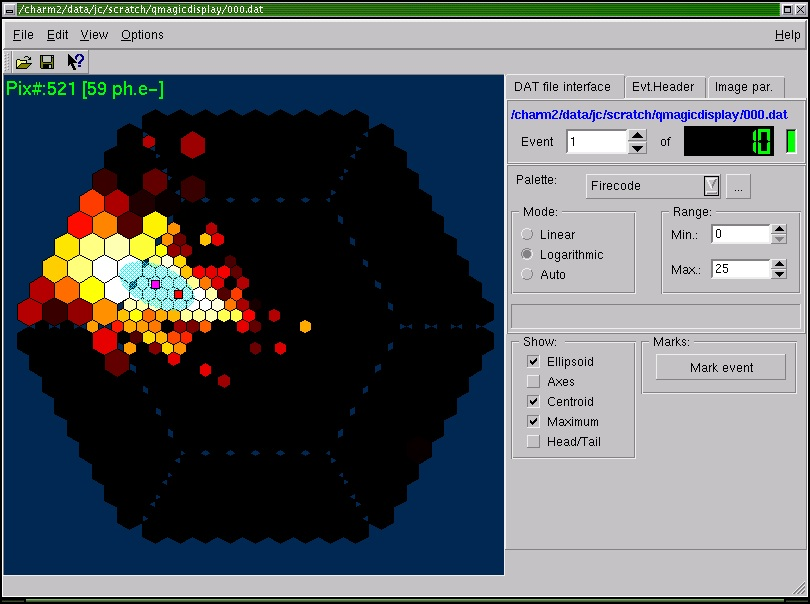
\includegraphics[width=\textwidth]{qmagicdisplay1}
  \caption{Imagen de una cascada gamma de $500\u{GeV}$ de energ'ia
    primaria, mostrada en el visualizador de sucesos creado para
    \MAGIC.}
  \label{fig:qmagicdisplay}
\end{figure}


\endinput
%
%% Local Variables:
%% mode:latex
%% TeX-master: t
%% End:

%%EOF
